\chapter{绪论}
\section{选题来源}
本论文选题是由指导老师推荐,和老师交流协商之后确定选题。
\section{意义和背景}
本文的目的是在理论上提供一个拓扑绝缘体的介绍。具体方法是从紧束缚模型出发,然后引入拓扑不变量并切实地对一些低维的拓扑模型做一些数值模拟,探索其有趣的物理性质。最后我们会对拓扑物理的一个前沿方向——高阶拓扑绝缘体做一些理论上的讨论和数值模拟。

拓扑物理是物理学中一个相对新颖的分支。有趣的是,它解决的最早问题可以追溯到19世纪。1879年,霍尔把一块材料通上电流,并在和电流垂直的方向上加上一个均匀的磁场。霍尔随后发现在同时垂直于电流和磁场方向上,材料产生了电势差\cite{hallOrigin}。这个电势差的物理来源可以用电磁学中的洛伦兹力来解释:电子在同时垂直速度和磁场方向上受到了一个力。在随后的一年,霍尔把上述材料换成了铁磁体,竟发现材料的霍尔电阻多了和正比磁化矢量成正比的一项\cite{hall2nd}。这一项要在百年后,即1980年代,利用能带的拓扑结构才得以解释。在这个年代附近的几十年里,拓扑理论还成功地解释了很多其他的霍尔现象 – 自旋霍尔效应,量子霍尔效应,量子反常霍尔效应(未确定)和量子自旋霍尔效应。对这些新奇物理现象的解释可以说是拓扑理论的胜利。不仅如此,拓扑理论还热衷于和其他物理分支结合,例如说冷原子模拟拓扑材料,超流体,超导体和量子计算。总之,拓扑理论是凝聚态中一个比较基础的理论,对整个凝聚态的发展以及对新材料的探索有重要的意义。而本文所要讨论和探索的低维拓扑模型又能很好地抓住拓扑物理的物理图像,从而提供一个较为清晰的介绍。
\section{国内外研究现状}
拓扑物理在历史上前中期的发展本质上就是对一系列霍尔效应的解释和预言的过程。1879年霍尔给一块材料加上电流,在与电流垂直方向上加了磁场\cite{hallOrigin}。这样当电子通过材料时会受到一个由磁场引起的洛伦兹力
\begin{equation}
\mathbf{F_L} = q \mathbf{v} \times \mathbf{B}
\end{equation}
其中q是电荷载体的电荷量,$\mathbf{v}$是电子速度,$\mathbf{B}$是磁感应强度。这个洛伦兹力的方向同时与电流方向和磁场方向垂直,就会导致电子被拉到材料的侧面从而形成堆积,进而在侧面形成一个电势差(霍尔电压)。稳定时洛伦兹力和侧面所形成的电场力会达到平衡状态
\begin{equation}
 q \mathbf{v} \times \mathbf{B} = q \mathbf{E}
\end{equation}
从而可以得到霍尔电压
\begin{equation}
  V_H = EW
  \end{equation}
其中W是材料的宽度。霍尔电阻被定义为
\begin{equation}
  R_L B = \frac{V_H}{I} = \frac{B}{q\rho_e}
\end{equation}
这里$\rho_e$是电荷载体密度。在随后的一年,霍尔把材料换成了铁磁性材料,发现霍尔电阻除了上面那个由洛伦兹力引起的一项外还有额外的,和磁化矢量成正比的一项
\begin{equation}
R_H = R_L B + R_A M 
\end{equation}
这多出来的一项需要一个世纪后用拓扑理论有关的知识才能解释。这个效应又被称作反常霍尔效应。

反常霍尔效应的其实是由于存在自旋有关的效应使电子侧向移动。总的来说,这个自旋有关的效应来源有两种:一种是外因——自旋依赖的无序带电载体碰撞;一种是内因——材料的特殊能带结构。这种特殊能带结构可以用一个拓扑概念:Berry phase 来描述\cite{abnomalHall}。从经典图像来看,电子会受到一个自旋轨道力或者自旋横向力,从而往侧面移动。这种力的来源是自旋电流而非洛伦兹力所用到的电荷电流\cite{spinCurrent}。自旋向上的电子会被移动到另外一侧,而向下的电子会被移动到另外一侧。在铁磁材料中,自旋向上和向下的电子数目不相等,从而造成材料侧面电荷堆积量不均,因此在霍尔电阻上会有额外的一项出现。
  
反常霍尔效应的出现依赖外部磁场,但是自旋霍尔效应却并不依赖。自旋霍尔效应首先由俄
罗斯物理学家Dyakonov 和 Perel在1971年提出\cite{rassian, rassian2}。和反常霍尔效应类似,他们认为自旋霍尔效应的来源是自旋方向不同的电子会在材料两个侧面有不均匀堆积。但是没了磁场,自旋方向不同的电子为什么会堆积成了一个问题。一开始物理学家认为这是由于材料不干净,在碰撞中会发生“特异性”的散射:不同自旋方向的电子会被散射到不同方向\cite{scatterForHall}。但是在2003年,两个独立的课题组展示了具有自旋耦合的能带就能产生横向电流,从而解释自旋霍尔效应,而不需要用到碰撞\cite{indepenSpinHall}。自选霍尔效应同样可以用拓扑理论解释。
  
近代以来众多霍尔效应里最出名的当属整数阶量子霍尔效应。1980年,von Klitzing, dorda和pepper在实验上首次发现了这个效应\cite{intHall}。他们制成了一种特殊的半导体。这个半导体中间有一个分界线,分界线的两侧分别为不同的物理材料。在材料上加上一些电压的控制,在分界线附近就能够形成二维电子气体。他们往这个电子气体加上强磁场,发现系统会产生一个霍尔电导(霍尔电阻的倒数)。这个电导随着磁场的加强会出现平台效应:在某一段磁场变化范围内电导不发生变化(图\ref{integerHall})。霍尔电导的公式为
\begin {figure}[tbp]
\centering 
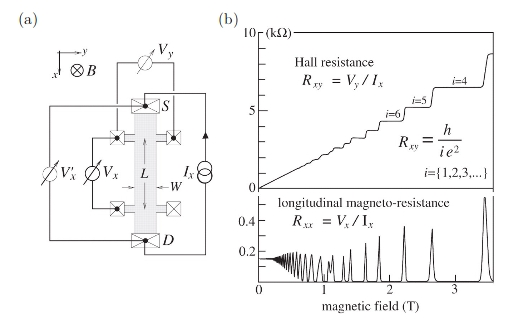
\includegraphics[width=12cm]{./images/hallR.jpg} 
\caption{(a)实验装置草图。磁场B垂直纸面向里,电流通过体系的y方向。有装置测量y和x方向的电压。(b)霍尔电阻和径向(y方向)电阻随磁场变化图像。\cite{hallR}}
\label{integerHall}
% J. Weis and K. von Klitzing. Metrology and microscopicpicture of the integer quantum Hall effect.Phil. Trans. R.Soc., 369:3954–3974, 2011.  doi:10.1098/rsta.2011.0198.
\end {figure}
\begin{equation}
  \sigma_H = \nu e^2 / h
  \label{hallInduc1}
\end{equation}
其中$\mu$是非零自然数,h是普朗克常数。整数阶霍尔效应可以通过朗道能级来解释。朗道能级是自由电子在磁场中产生的能级,它的哈密顿量为
\begin{equation}
  H = \frac{1}{2m}[(\hat{p_x} - e B_y)^2 + \hat{p_y}^2 + \hat{p_z}^2]
\end{equation}
$\hat{p}$是粒子的动量方向,$m$是粒子质量。由此可以通过解薛定谔方程来得到朗道能级。
\begin{equation}
  E = (n + \frac{1}{2})\hbar \omega_c + \frac{\hbar^2 k_z^2}{2m}, n = 0, 1, 2...
\end{equation}
其中回旋频率
\begin{equation}
  \omega_c = \frac{eB}{m}
\end{equation}
而$k_z$的取值范围为
\begin{equation}
  k_z = \frac{2 \pi}{L} n_z, n_z \mbox{ is an integer}
\end{equation}
L是材料长度。当磁场增大时,系统的能级会进行放缩。而费米能级不变。这样结果就是费米能级在磁场增大时间断性地扫过朗道能级和能级间隙。当费米能级处于能级间隙时,电子填充状态不变,则为平台。费米能级扫过某个朗道能级时,电子填充或者逃开能级,这就产生了电导率的变化。现在物理学家已经认识到式(\ref{hallInduc1})里的$\nu$整数实际上是一个拓扑不变量\cite{nuIsTopo}。这个不变量对具体材料的几何结构不敏感。

这里还有一个更为直观的解释。电子在均匀磁场中会受到洛伦兹力而做圆周运动。圆周的半
径约为$R_n = \sqrt{\frac{\hbar}{eB}(2 n + 1)}$。一部分电子处于边界处,会在完成整个圆周运动之前撞到边界,被反弹回来。这就导致了电子沿着边界会有移动。这种运动状态又被称作是边界态。其实这种边界态是受到拓扑对称保护的,即使对材料进行掺杂,例如说在边界处加一些“阻碍”,也不会对边界态产生影响。

1982年,Tsui,Stormer和Gossard对量子霍尔效应的研究更进了一步。他们发现了分数阶的
量子霍尔效应\cite{fracHall}。在这种效应里,霍尔电导的系数$\nu$不是整数,而是分数。分数量子霍尔
效应的原理比较复杂。电子和电子间的相互作用在这个效应里是主要因素。Laughlin提出了
一个和$\nu = 1 / 3$有关的新型多体凝聚态\cite{newCondense}。这种凝聚态由于库伦作用,可以被等价为具有电荷为e/3的一种伪粒子。因此,分数阶的量子霍尔效应可以被解释为一种伪粒子的整数霍尔效应。在1988年,Jainendra K. Jain进一步发展了这个观点,提出这种新型凝聚态是电子和量子化的磁通量结合的结果,又被称作composite fermions\cite{compositeF}。现在我们知道分数阶的量子霍尔效应其实是composite fermions的一种拓扑相。这种相破坏了材料的时间反演对称。
  
整数阶量子效应的出现并不一定需要一个方向上的强磁场。1988年Haldane认为给材料施加周期性的磁通量,即使没有切实的磁场,也会出现整数量子霍尔效应\cite{haldane}。就像人们把无磁场情况下的霍尔效应命名为反常霍尔效应,我们也把这种无磁场情况叫做反常量子霍尔效应。反常量子霍尔效应发生的机理是材料特殊的能带结构,而不是简单的朗道能级在磁场中的变化。后来,物理学家又发现甚至周期性的磁通量也是不必要的,只需要铁磁性材料中的强自旋-轨道耦合即可。反常量子霍尔效应的电导可以用Berry curvature在动量空间的积分或者Chern数来表示\cite{anomaQt}。一个非0的Chern数表示非平凡的拓扑材料。而Haldane模型首次实现了零磁场下的非零chern数。在反常量子霍尔效应之后还有量子自旋霍尔效应,最后演化出来现今的一块物理研究的前沿—拓扑绝缘体。这些霍尔效应们的关系可以被总结为图\ref{hallRelation}
  
 \begin {figure}[btp]
\centering 
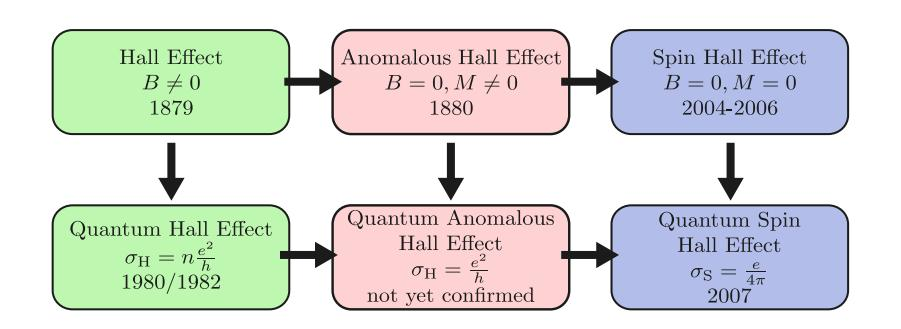
\includegraphics[width=12cm]{./images/hallRelation.jpg} 
\caption{霍尔效应和量子霍尔效应的发展以及他们的相互关系。$B$表示外加的磁场,$M$是铁磁体的磁化强度。最下面一行的年代表示这个效应被发现的年份。$\simga_H$是霍尔电导,$\sigma_S$是自旋霍尔电导。\cite{}}
\label{hallRelation}
\end {figure} 
% ref: topotext book
  
 \section{结构安排}
 论文的目的是对低维拓扑材料理论做一个比较基础的介绍。因此文章会开始会在现今本科生所学的固体物理之上介绍紧束缚模型,然后再引入一些和拓扑有关的概念,进而求解一些简单的低维拓扑模型,最后介绍一个比较前沿的研究—高阶拓扑绝缘体。具体来说文章可以被分为以下几部分:
 
第一部分:介绍紧束缚模型,包括如何从图像上的晶格相互作用得到其哈密顿量,进而得到能带。这个求解技术会在后面对拓扑模型的求解中用到。

第二部分:介绍拓扑物理的一些基本概念。Berry phase的概念可以从含时薛定谔方程出发得到。之后还会得到从Berry phase引入的其他物理量,包括Berry connection,Berry curvature,chern number等。

第三部分:这部分会解析或者数值求解一些低维的模型从而揭示chern number背后的物理。

第四部分:这部分我们会介绍高阶拓扑绝缘体。包括介绍具体的模型和数值模拟一些它的性质。

第五部分:对文章的工作作出总结和展望。